\subsection{OSN 19 Системы программирования. Основные компоненты систем программирования, схема их функционирования. Общая схема работы компилятора. Основные методы, используемые при построении компиляторов.}

\begin{itemize}
    \item \textbf{Системой программирования} называется комплекс программных средств, предназначенных для поддержки программного продукта на протяжении всего жизненного цикла этого продукта.
    \item \textbf{Этапы жизненного цикла} программного продукта: разработка, сопровождение, эксплуатация.
    \item \textbf{Этапы разработки программного продукта}
        анализ требований,
        проектирование,
        написание текста программ (``кодирование''),
        трансляция, компоновка/интеграция (связывание частей программы в единую систему),
        верификация (процесс проверки на правильность), тестирование (обнаружение дефектов посредством сравнения с эталоном) и отладка (процесс поиска причин дефектов и их устранение),
        документирование,
        внедрение,
        тиражирование,
        сопровождение (этот этап является повторением всех предыдущих).
    \item \textbf{Основные компоненты системы программирования:}
    \begin{enumerate}
        \item \textbf{Транслятор} переводит программы на исходном языке программирования в некоторый целевой язык.
        В случае, когда транслятор является компилятором, целевой язык --- язык ассемблера, машинный код или байт-код некоторый виртуальной машины.
        \item \textbf{Интерпретатор} выполняет программы без необходимости предварительной компиляции в машинный код.
        Может содержать \textbf{Just-in-Time} (\textbf{JIT}) компилятор, который транслирует программу в машинный код во время выполнения для оптимизации часто используемых участков кода.
        Если интерпретатор выполняет не исходный текст, а некоторое промежуточное представление (называемое байт-кодом), то интерпретатор называется виртуальной машиной.
        В этом случае для получения байт кода необходим отдельный транслятор.
        \item \textbf{Макрогенератор или макропроцессор} выполняет преобразование текста программы, выполняя замену вызовов макроопределений их определениями.
        Если макропроцессор входит в состав транслятора, его называют \textbf{Препроцессором}. В этом случае он выполняется непосредственно трансляцией кода в целевой язык.
        \item \textbf{Редактор текстов} используется для написания и редактирования исходного текста программ на языке программирования.
        \item \textbf{Редактор связей} или \textbf{компоновщик} используется для связывания между собой (по внешним данным) объектных модулей, порождаемых компилятором,
        а также файлов библиотек (которые являются наборами обьектных модулей внутри одного файла), входящих в состав СП.
        \item \textbf{Отладчик} используется для проверочных запусков программ и исправления ошибок. В нем обычно присутствуют такие возможности как интроспекция (получение типов данных) и анализ данных программы во время выполнения,
        остановка выполнения в определенной точке или при определенном условии, пошаговое выполнение программы и сопоставление машинного кода программы ее исходного кода при выполнении.
        \item \textbf{Библиотеки стандартных программ} облегчают работу программиста, используются на этапе трансляции и исполнения.
    \end{enumerate}
    \item \textbf{Дополнительные компоненты систем программирования:}
    \begin{enumerate}
        \item \textbf{Система контроля версий} для версионирования исходного текста ПП (git).
        \item \textbf{Средства конфигурирования} помогают создавать различные конфигурации ПП в зависимости от конкретных параметров системного окружения.
        \item \textbf{Система сборки} позволяет автоматизировать сборку ПО (maven)
        \item \textbf{Средства тестирования} помогают при составлении набора тестов, автоматического выполнения тестов.
        \item \textbf{Профилировщик} используется для анализа поведения программы и поиска критических участков кода, на которые затрачивается наиболее количество ресурсов (пример: анализ затрачиваемого на выполнение каждой функции времени, возможно в процентах от полного временем выполнения программы). Используется для оптимизации программ.
        \item \textbf{Справочная система} содержит справочные материалы по языку программирования и компонентам СП.
        \item \textbf{Инструменты для статического анализа кода} позволяет найти дефекты в программном коде без выполнения программы с помощью формальных методов.
        \item \textbf{Средства навигации по коду} позволяют более эффективно ориентироваться в коде и поддерживают, например, переход от вызова функции к ее определению.
        \item \textbf{Инструменты подготовки документации.} (Sphinx)
        \item \textbf{Система управление разработкой.}
    \end{enumerate}
\end{itemize}

В другой терминологии интерпретаторы также называют трансляторами.

В системе программирования должен обязательно присутствовать транслятор или интерпретатор.
также могут присутствовать оба. В этом случае они либо взаимозаменяемы (Например, tiny c compiler может либо интерпретировать Си, либо компилировать),
либо, если интерпретатор это виртуальная машина, должны использоваться одновременно (Например, java: javac+javavm).

\textbf{Схема функционирования компилятора} и \textit{часто применяемые алгоритмы (методы):}
\begin{enumerate}
    \item \textbf{Лексический анализ.} Лексический анализатор читает поток символов исходного текста программы и группирует эти символы в значащие последовательности -- \textbf{лексемы}.
    \textit{Используется разбор с использованием регулярных грамматик для преобразования потока символов в поток лексейм.}
    \item \textbf{Синтаксический анализ.} Синтаксический анализатор формирует из последовательности лексем (токенов) промежуточное представление программы (синтаксическое дерево, AST, dop24).
    	\textit{Используются алгоритмы разбора грамматик, наиболее эффективные для данной грамматики, например, рекурсивный спуск, LL(1), LR(1) или, для отдельных частей грамматики, регулярные выражения.}
    \item \textbf{Семантический анализ.} Семантический анализатор проверяет исходную программу на семантическую согласованность с определением языка (например, проверка типов). \textit{Используются различные обходы графов (DFS, BFS) и их пометка}
    \item \textbf{Генерация промежуточного кода.} Перевод AST в некоторое промежуточное представление, на котором удобнее производить оптимизации.
    	\textit{Часто применяется SSA-форма (single static assignment), в которой каждой переменной можно присвоить значение лишь единожды. Для ее построения используется обход графа для генерации трехадресного кода и алгоритм преобразования генерации $\phi$-функций для преобразования в SSA.}
    \item \textbf{Машинно-независимая оптимизация.} Серия трансформаций промежуточного кода с целью увеличения скорости его работы на целевом процессоре с сохранением семантики работы программы.
    	\textit{Используются различные алгоритмы работы с графами, см. билеты dop25, dop26.}
    \item \textbf{Машинно-зависимая оптимизация и генерация кода.} Трансляция промежуточного представления компилятора в машинный код целевого процессора с применением наиболее эффективных для целевой машины инструкций и генерация объектного файла. \textit{Также используются различные алгоритмы работы с графами. Для выбора инструкций --- сопоставления подграфа с образцом (алгоритм пытается найти фрагменты графа, которые некоторой машинной инструкции, например для \texttt{$(x << n) | (x >> (32 - n))$} может быть использован циклический сдвиг вправо) и использования знаний компилятора для выбора наиболее эффективной инструкции для данной инструкции промежуточного кода.}
\end{enumerate}

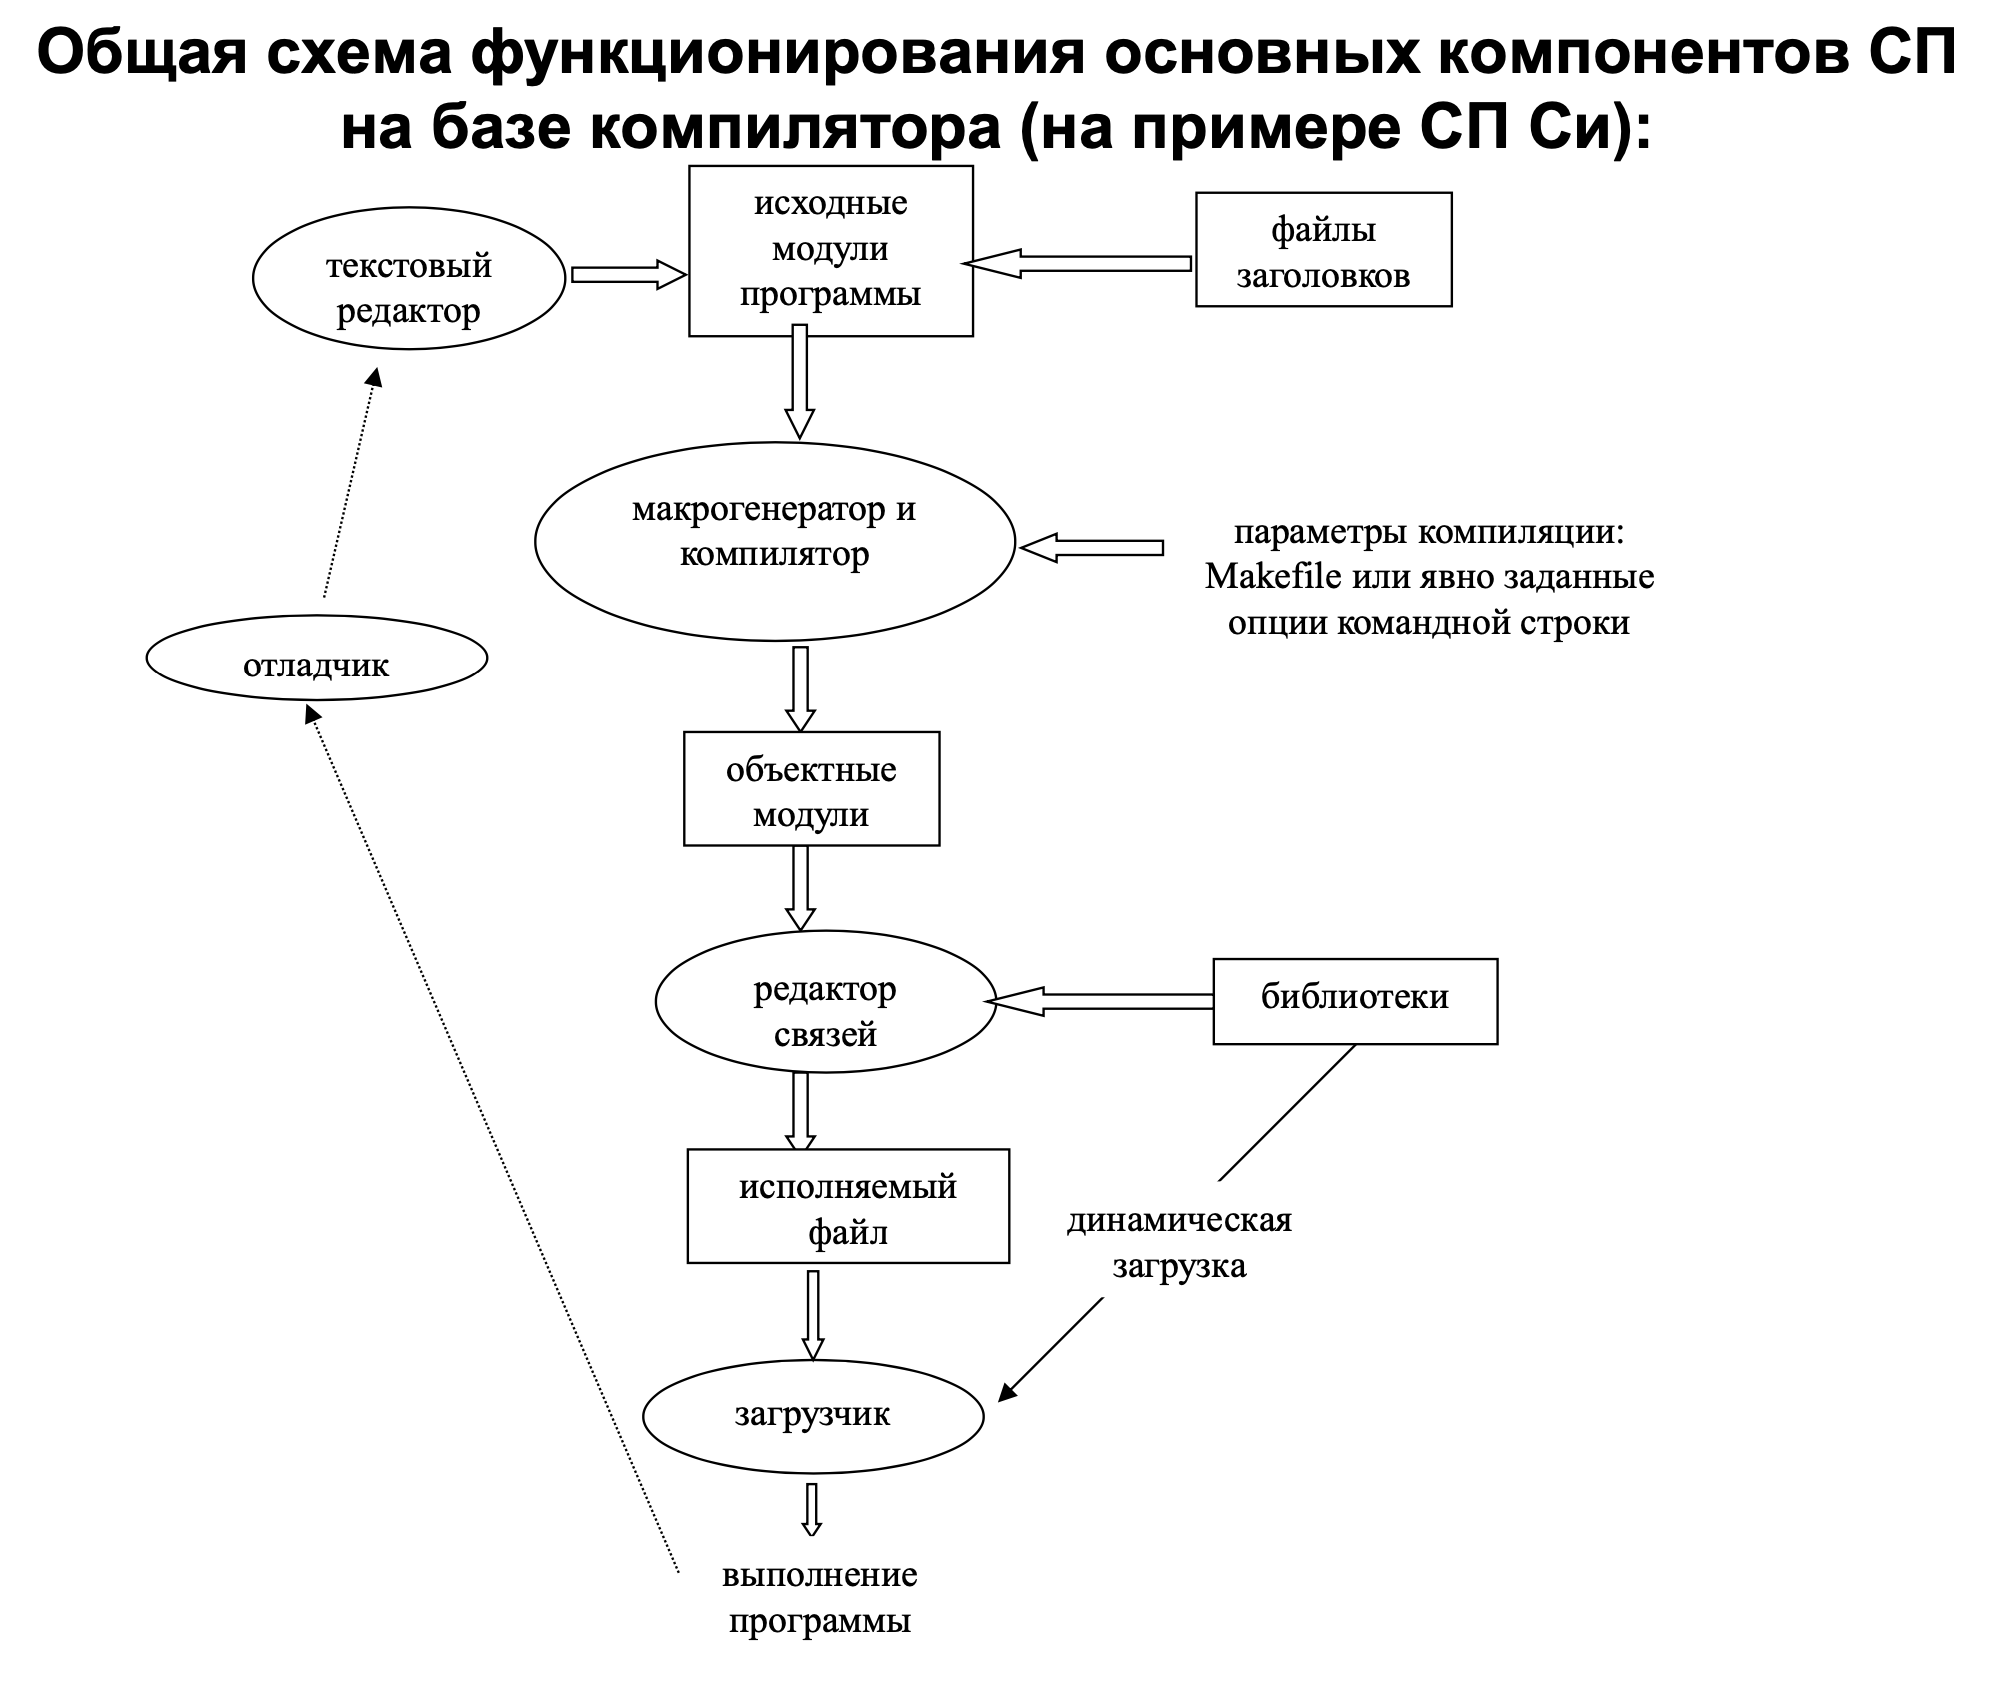
\includegraphics[width=0.5\columnwidth]{pics/scheme_compiler.png}%
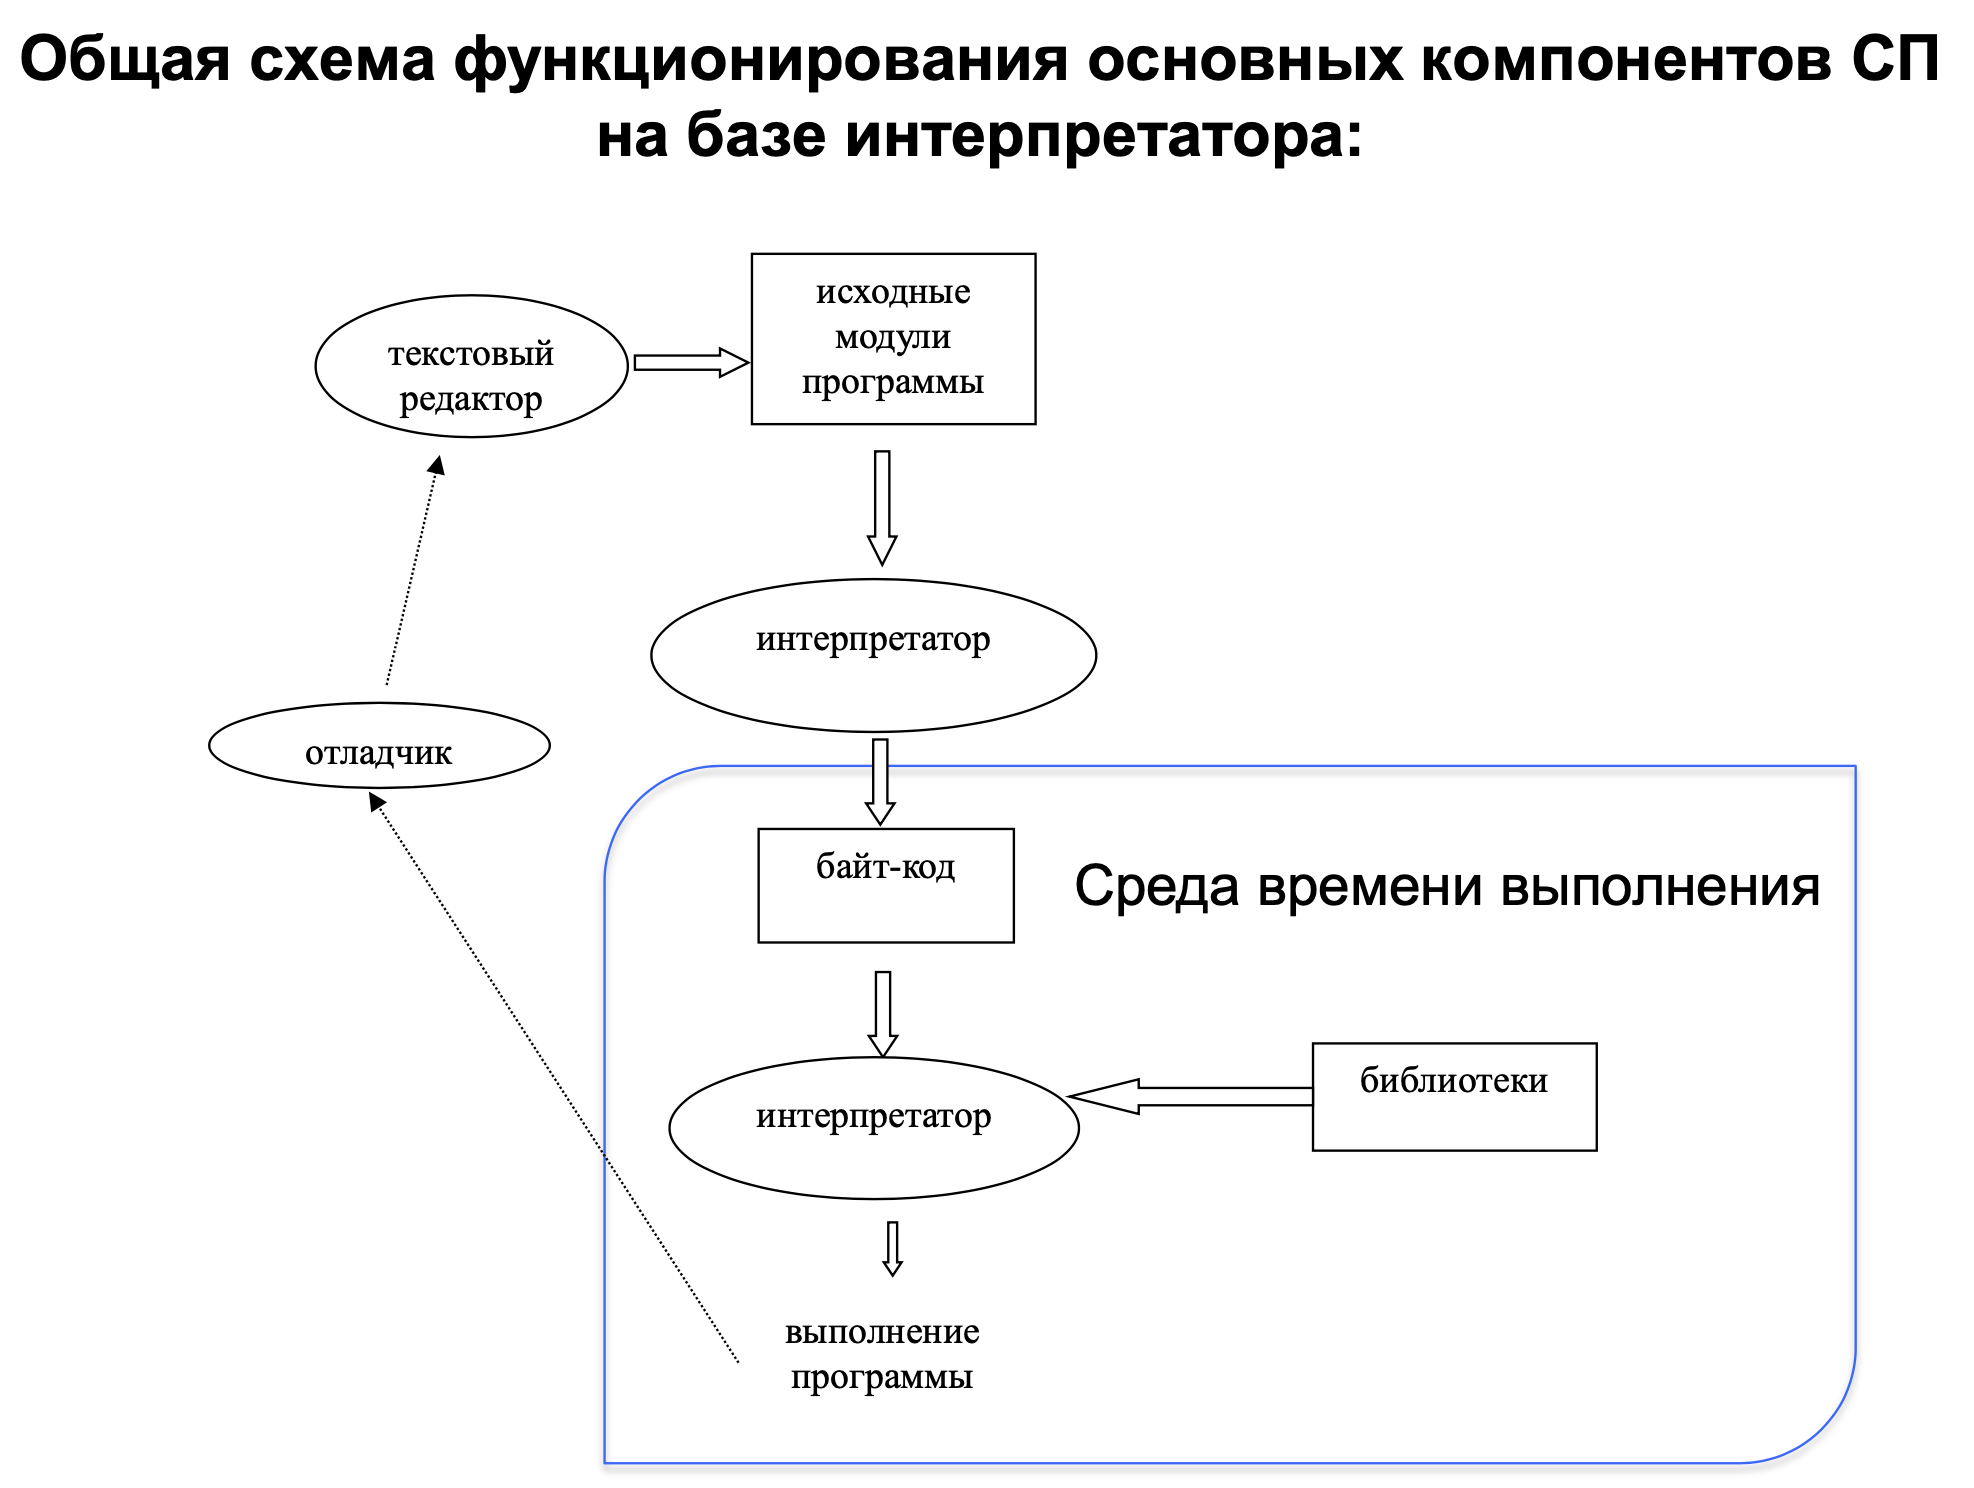
\includegraphics[width=0.5\columnwidth]{pics/scheme_interpret.png}

% -------- source --------
% \bigbreak
% [\cite[page 69-96]{replace_me}]
